\chapter{Droga do rozproszenia}
\label{cha:rozproszenie}

Prawo Moore'a \cite{moore1998cramming}, wspominające o podwajaniu ilości tranzystorów w procesorach, często parafrazowane jako podwajanie ich mocy obliczeniowej, przestaje działać, podczas gdy złożoność problemów i ilość użytkowników szerokopasmowego internetu rośnie. 
Próba skalowania wertykalnego -- polegającego na wzmacnianiu pojedynczych węzłów -- przestaje zdawać próbę czasu.

Problem posiada także drugą stronę -- nie wszyscy użytkownicy internetu mogą pozwolić sobie na łącze szerokopasmowe. Szacuje się, że w roku 2017 dostęp do internetu posiada ponad połowa populacji świata; sam wzrost ilości użytkowników sieci Web z Afryki od roku 2000 do 2017 wynosi aż 8503.1\% \cite{webStats} – znaczną część tych połączeń stanowią jednak połączenia starych generacji sieci komórkowej, o znacznie ograniczonej przepustowości i ogromnych latencjach. Każdy kolejny węzeł niezbędny do połączenia użytkownika z serwerem końcowym może dokładać cennych milisekund czasu odpowiedzi. 

Autorzy IPFS zauważają w swojej pracy \cite{ipfsWP} także inne słabości obecnego internetu – sieć oparta o HTTP jest w prawdzie zdecentralizowana, jako iż treści rozdzielane są pomiędzy miliony węzłów, od gigantycznej sieci Amazon Web Services aż po mikroserwery stojące w domach pasjonatów; brakuje jej jednak faktycznego rozproszenia: ta infrastruktura nie jest gotowa na przyjmowanie gigantycznego ruchu, nie jest w stanie efektywnie przechowywać i udostępniać wielkich zestawów danych; jest również podatna na znikanie danych, jako iż awaria pojedynczego dysku twardego może zatrzymać udostępnianie całej witryny. 


\section{Zarys historyczny}
\label{sec:teoriaRozproszenia}
W świecie informatyki szybko wyewoluowały \textbf{rozwiązania współbieżne}. Istnienie wielu wątków -- niezależnych od siebie logicznie toków wywołań, operujących na wspólnej pamięci -- rozwiązywało takie problemy, jak nierówny rozmiar żądań -- działający sekwencyjnie serwer blokowałby się przy poleceniach zajmujących więcej czasu. Dzięki przeplataniu wątków można uniknąć tej sytuacji, a także pozwolić na iluzję symultaniczności -- mimo korzystania z jednego procesora, polecenia wykonywane są {\em pseudorównolegle}, co pozwala między innymi na responsywność interfejsów użytkownika.

Upowszechnienie się komputerów wieloprocesorowych i procesorów wielordzeniowych zaowocowało rozwojem \textbf{obliczeń równoległych}. Istotne jest rozgraniczenie tych dwóch pojęć -- współbieżność jest raczej paradygmatem, sposobem strukturyzacji oprogramowania w sposób, który pozwala na wykonywanie wielu poleceń niezależnie i jednocześnie; równoległość z kolei to możliwość uruchamiania tego typu oprogramowania w tym samym czasie, dzięki mnogiej liczbie procesorów \cite{concurrencyGo}.

Współbieżność i równoległość rozwiązują problemy obciążenia, ułatwiając operacje na współdzielonej pamięci. Istnieją całe klasy algorytmów naturalnie podatnych zrównoleglaniu: mapowanie, grupowanie, przeszukiwanie czy sortowanie są jednymi z przykładów. Choć w niektórych przypadkach adaptacja algorytmu wymaga jego konkretnej modyfikacji, możliwość rozwiązywania składowych problemu jako niezależnych wątków znacznie przyspiesza wykonanie w środowiskach wieloprocesorowych \cite{parallelAlgo}.


Skalowanie rozwiązań tego typu może jednak stać się kłopotliwe z powodu kosztów -- niezbędne są duże ilości pamięci RAM i szybkie dyski; cierpi też niezawodność systemu, gdyż jego działanie pozostaje kompletnie uzależnione od utrzymania przy życiu konkretnego komputera. Jeśli komputer musi też propagować dane w sieci, cała komunikacja spoczywa na nim -- i wydajność jego łącza może zawieść w przypadku szczytów obciążenia.

Remedium dla powyższych problemów jest próba rozdzielenia pracy pomiędzy wiele komputerów -- tu pojawia się \textbf{decentralizacja}, podział problemu na podproblemy, którymi zarządzać mogą mniejsze węzły główne, mające dostęp do węzłów roboczych. To rozwiązanie stawia też nowe wyzwania przed projektantami oprogramowania, którzy nie mogą już polegać na współdzielonej pamięci -- dane muszą być przekazywane jakąś sieciową metodą komunikacji.

Obliczenia decentralizowane uznać można za podklasę \textbf{obliczeń rozproszonych}. Dla potrzeb tej pracy, obliczenia rozproszone zdefiniowane zostaną jako prowadzone przez w pełni autonomiczne węzły, które dzielą między sobą pracę i radzą sobie z pojawianiem się i znikaniem kolejnych elementów sieci; innymi słowy, w warstwie logicznej system rozproszony powinien zachowywać się identycznie zarówno przy istnieniu zaledwie jednego węzła sieci, jak i przy milionie -- różnicą powinien być wyłącznie spadek wydajności systemu.


\begin{figure}[h]
	\centering
	\begin{subfigure}{0.4\textwidth}
		\centering
		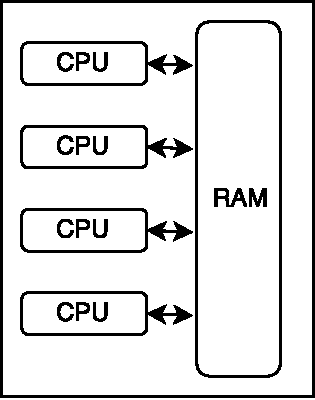
\includegraphics[scale=0.6]{parallel.pdf}
		\subcaption{\label{subfigure_a}}
	\end{subfigure}
	\begin{subfigure}{0.5\textwidth}
		\centering
		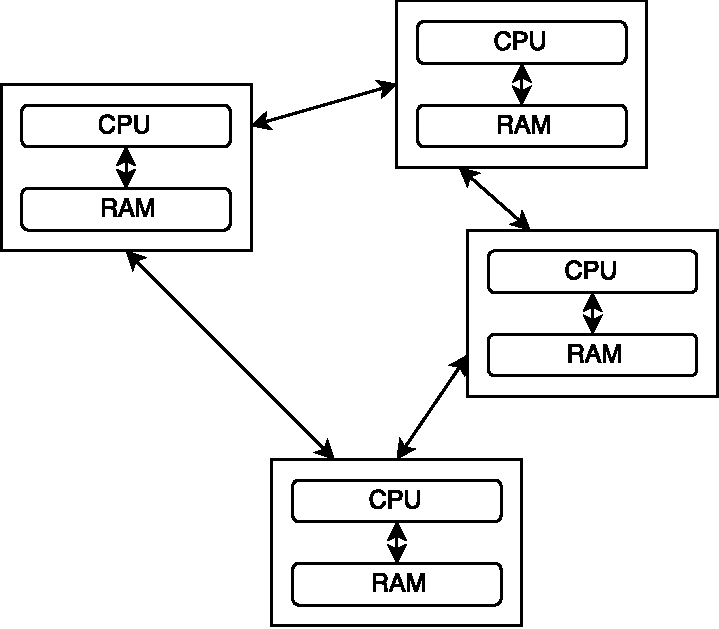
\includegraphics[scale=0.5]{distributed.pdf}
		\subcaption{\label{subfigure_b}}
	\end{subfigure}
	\begin{subfigure}{0.6\textwidth}
		\centering
		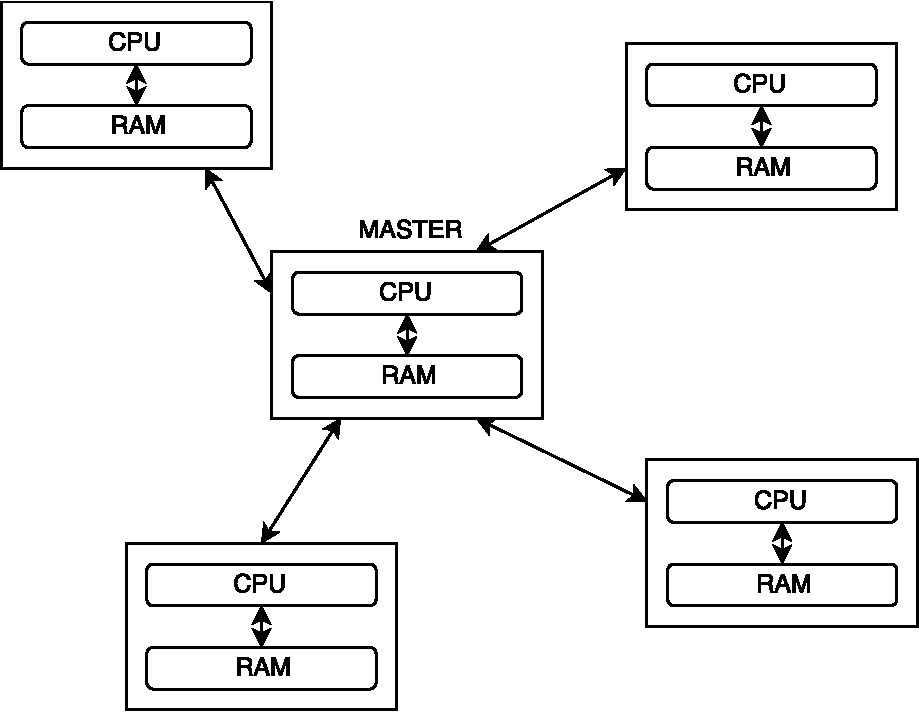
\includegraphics[scale=0.5]{decentralized.pdf}
		\subcaption{\label{subfigure_c}}
	\end{subfigure}
	
	\caption{\label{fig:concurrentVsParalell}Wizualizacja różnicy pomiędzy systemem równoległym \protect\subref{subfigure_a}, rozproszonym \protect\subref{subfigure_b} i zdecentralizowanym \protect\subref{subfigure_c}.}

\end{figure}

\section{Narzędzia rozpraszania danych}
\label{sec:narzedzia}
Najbardziej istotnym problemem z dziedziny rozproszenia dla systemu dHTTP jest rozproszenie danych -- próba propagowania informacji pomiędzy wiele węzłów sieci, w celach takich jak podniesienie wydajności, obniżenie kosztów, zwiększenie dostępności czy zapewnienie trwałości informacji.

Dobrym przykładem rozwiązania rozproszonego w operacjach na danych jest system kontroli wersji \texttt{git}.
Został stworzony przez Linusa Torvaldsa, autora jądra Linux, jako otwarta alternatywa dla systemu BitKeeper, który wycofał z dystrybucji darmową wersję swojej aplikacji projektom open source.
\texttt{git} jest projektem czysto rozproszonym -- każdy użytkownik posiada kompletną kopię repozytorium, z informacjami o wszystkich zmianach i ich autorach, na której może wykonywać operacje w trybie offline; nie jest uzależniony od istnienia centralnego serwera (choć jego stosowanie jest powszechne; każdy użytkownik o aktualnej wersji repozytorium mógłby jednak pełnić jego rolę), a zmiany mogą być propagowane na różne sposoby, takie jak email czy przekazywanie łat w formie tekstowej. Dzięki swojej wydajności i silne zdecentralizowanemu designowi, \texttt{git} jest chętnie wybieranym rozwiązaniem nie tylko w środowiskach programistów, a w środowiskach profesjonalnych wypiera konkurencyjne rozwiązania, takie jak Apache Subversion czy CVS \cite{ram2013git}.

Nie zawsze jednak motywacje stojące za rozpraszaniem danych poza centralne serwery były szczytne. Duży wpływ na rozwój technik stosowanych obecnie -- w tym wykorzystywanych przez dHTTP -- mają rozwiązania rozpowszechnione głównie przez piractwo komputerowe. Systemy peer-to-peer -- polegające na współpracy równorzędnych węzłów -- zostały spopularyzowane dzięki aplikacji Napster, która w roku 2001 zgromadziła około 80 milionów użytkowników. Zaprojektowana jako system współdzielenia plików, wyspecjalizowała się w łatwym udostępnianiu plików MP3. Napster wzburzył wiele kontrowersji -- w systemie pojawiały się niewydane jeszcze utwory znanych artystów, prowadząc do milionowych strat i procesu, który pogrążył działanie systemu.
Problemem Napstera była architektura oparta o centralny serwer indeksujący -- każdy podpięty węzeł informował o posiadanych przez siebie plikach, a punkt centralny był niezbędny do przeszukiwania bazy plików i przekazywania poleceń pobrania innym węzłom. To rozwiązanie stanowiło słaby punkt sieci, i pozwoliło obciążyć twórców programu odpowiedzialnością za szerzone w nim treści.

Błędy Napstera zostały zauważone przy kolejnych projektach tego typu. Gnutella, chcąc uniknąć istnienia {\em single point of failure}\footnote{Punkt sieci, którego awaria powoduje zatrzymanie pracy całego systemu.}, działała na zasadzie rozgłaszania poleceń użytkowników do wszystkich maszyn w sieci, co owocowało jednak drastycznym spadkiem wydajności \cite{measuringNapsterGnutella}.

Alternatywne podejście podjęte zostało przez sieć Freenet, gdzie zastosowano heurystyczny routing oparty o klucze; każdy plik otrzymuje klucz, a podobne klucze lokowane były na zbliżonych do siebie węzłach, dzięki czemu przeszukiwanie sieci nie wymagało punktu centralnego, a polecenia kierowane były w sposób niewymagający wielu przeskoków. Niestety, ta metoda nie gwarantowała znalezienia danych \cite{searchingInSmallWorld}.

Chcąc pogodzić kwestie bezpieczeństwa, wydajności i spójności systemu, rozpoczęte zostały intensywne prace nad rozproszonymi tablicami haszującymi (distributed hash table -- \textbf{DHT}). To rozwiązanie pozwala na trzymanie dużych ilości informacji w sposób kompletnie rozproszony -- wszystkie węzły sieci znają zestaw kluczy, stanowiących {\em de facto} adresy danych, pozwalające użytkownikom na przeszukania; znalezienie węzłów trzymających właściwe dane jest umożliwione dzięki ich opartemu o klucze sposobie identyfikacji. Choć przechowywanie tablicy DHT jest dodatkowym kosztem obciążającym system, i wymagane jest ustalenie wspólnych funkcji haszujących, przy właściwej konfiguracji to rozwiązanie pozwala na obsługę całej sieci danych bez serwerów pośredniczących.

\section{Podstawa projektu}
\label{sec:podstawaProjektu}

Wspomniane rozwiązania stanowią kanwę dla projektu IPFS \cite{ipfsWP}, który stara się tworzyć efektywny, realnie rozproszony system plików, obsługujący gigantyczne zasoby danych z niskimi latencjami, redundancją danych i bez wymogu zaufania uczestnikom sieci.  Dane przechowywane są w drzewie Merkla, dzięki czemu przeszukiwanie sieci ma niską złożoność obliczeniową. Projekt skupia się na warstwie infrastruktury – po stronie użytkowej przypomina nieco system kontroli wersji \texttt{git}, a dane indeksowane są dzięki sumom kontrolnym, i ich adresy to wieloznakowe hasze. Takie podejście doskonale sprawdza się w skryptach i przy pracach prowadzonych przez ludzi obytych z tego typu narzędziami, nie jest to jednak system przyjazny użytkownikom domowym.

Celem tej pracy jest adaptacja dokonań projektu IPFS jako {\em przezroczysty} system wsparcia HTTP. W swoim założeniu, system nie może próbować zastąpić istniejących rozwiązań. Internet w obecnym kształcie nie jest gotowy na rewolucje – przykładem może być poziom przyjęcia się IPv6 \cite{googleipv6}, następnej generacji protokołu IP, która ma między innymi rozwiązać problem rozmiaru puli adresów. Brak realnej kompatybilności wstecznej sprawia, że konieczne są rozwiązania przejściowe. dHTTP jest bardziej nakładką, rozwinięciem obecnych rozwiązań -- współżyje z nimi -- co daje perspektywy spokojnego przyjęcia takiego rozwiązania przez rynek.

IPFS posiada wzorcową implementację w języku Go, i jest podstawą stosu sieciowego \texttt{libp2p}. Zbiór bibliotek udostępniony w projekcie \texttt{js-libp2p} stanowi fundament projektu dHTTP, który, dzięki natywnej implementacji w JavaScripcie, może być w pełni uruchamialny z poziomu przeglądarki.
